This section presents the evolution of optical fibre (OF) deployments, from the Points-Of-Presence (POPs) to the end users. POPs are covered in Section~\ref{sec:POPs}.

\subsection{Pilot's deployments}
\label{dep_pilots}

During the third reporting period\footnote{NOTE: Commons for Europe project has three reporting periods: Nov 2012 - Oct 2013, Nov 2012 - Oct 2013 and Nov 2013 - Oct 2014. In this document they can also be referred as fist year (Y1), second year (Y2) and third year (Y3), or simply 2012, 2013 and 2014.}, \emph{Gurb}'s pilot, the most developed of the three pilots, has kept growing steadily in terms of new users connected, in \emph{Vic}'s the PoP has been consolidated through the addition of new connections to the intial ones deployed in Y2, and in \emph{Rub\'{i}}, a pilot categorised as "blocked" by the end of the first year, the opportunity for retaking it appeared in Y2 has produced some tengible results during the current reporting period.


\FloatBarrier

\subsubsection{Gurb}
\label{dep_gurb}

Gurb, the first OF initiative to be put into practice, was started two years before Commons for Europe (C4EU) project begun. The subsequent deployments in other areas have greatly benefited from the problems solved, the procedures developed and the knowledge gathered during the execution of this pilot. The first iteration, which finalised before C4EU was started, proved that the commons model being used for WiFi deployments was also adequate for OF deployments. The second iteration, carried out during Y1 and Y2, focused on rural deployments, showing that model was not only valid for core infrastructure (i.e. rising the PoP and make the initial connections), but also to reach end-users. The third iteration, Y3, carried out at the urban area of the town evidenced that the model is also suitable for this sort of areas. During this iteration an option to reduce the entry costs and to boost new deployment areas has been developed and put in practice. Now the users interested in getting OF connection can decide between the model already used for the former iterations, that is to say, wait until a project for covering their area consolidates and then pay the whole connectivity costs (around 1.500\euro{} for rural deployments and around 750\euro{} for urban deployments) at once, or to declare their interest and support for a future deployment by paying a small monthly amount of money (at the moment 20\euro{}/month) as payment on account. This way the professionals have budget in advance which makes possible to undertake smaller projects, thus, fulfilling users' demands earlier on average. Once the connection is delivered to the users the remaining costs can be cleared or refinanced. This way the entry costs can be reduced up to a total amount of 40\euro{} a month (20\euro{}/month for the connectivity -Internet access included- and 20\euro{}/month for financing the deployment costs).

Table~\ref{tab:gurb} summarises the state of the \emph{Gurb}'s pilot at the end of the third reporting period. 

\begin{table}[H]\small
  \begin{center}
    \begin{tabular}{|l|c|}
      \hline
      \multicolumn{2}{|c|}{\textbf{OF deployment of \emph{Gurb}'s Pilot (Oct. 2014)}} \\
      \hline
      \hline
      Users already connected & 61 \\
      \hline
      Users in the waiting list & 25 \\
      \hline
      Unsubscribed users & 0 \\
      \hline
      Km of OF deployed & 30 \\
      \hline
      Topology & PoP, rural, urban \\
      \hline
    \end{tabular}
    \caption[Gurb pilot - state at the end of C4EU project (Oct. 2014)]{Gurb pilot - state at the end of C4EU project (Oct. 2014).}
    \label{tab:gurb}
  \end{center}
\end{table}

\figurename~\ref{fig:map_gurbVic_2014} shows a general view of Gurb's and Vic's deployments. Green are lines are existing fibres by October 2014. Yellow ones are planned deployments to be executed before May 2015. Purple lines are circuits owned by the municipality of Vic. \figurename~\ref{fig:map_gurb_2014} is a detailed view of the urban area covered during this last year.

\begin{figure}[H]
  \centering
  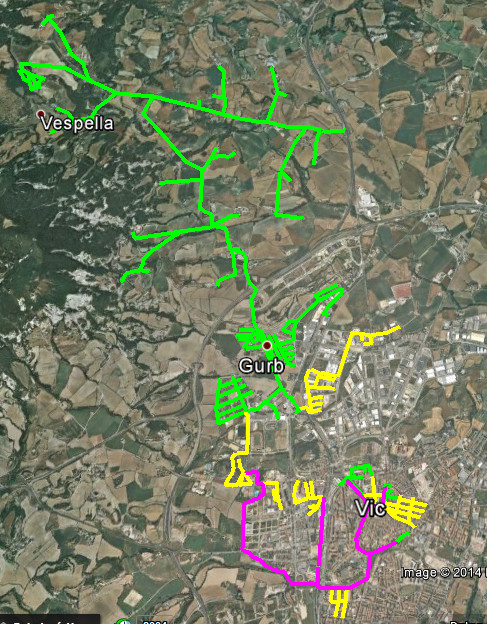
\includegraphics[width=0.95\linewidth]{sect2/figures/map_gurbVic_2014.jpg}
  \caption[Gurb's and Vic's pilot - general OF deployment map at the end of C4EU project (Oct. 2014)]{General OF deployment of Gurb's and Vic's pilots at the end of C4EU project (Oct. 2014). Green are lines are existing fibres by October 2014. Yellow ones are planned deployments to be executed before May 2015. Purple lines are circuits owned by the municipality of Vic.}
  \label{fig:map_gurbVic_2014}
\end{figure}

\begin{figure}[H]
  \centering
  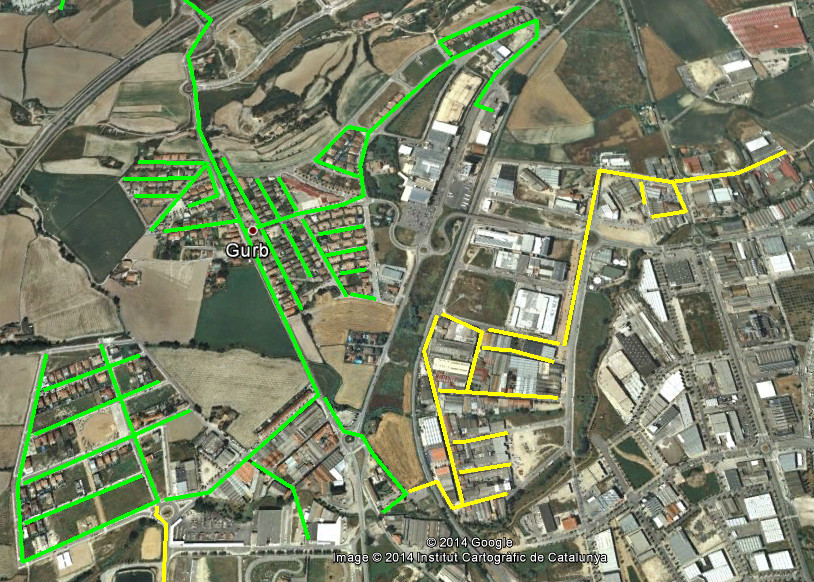
\includegraphics[width=0.95\linewidth]{sect2/figures/map_gurb_2014.jpg}
  \caption[Gurb pilot - OF deployment of 2014 in an urban area]{OF deployment of 2014 in an urban area.}
  \label{fig:map_gurb_2014}
\end{figure}

Pictures of \figurename~\ref{fig:gurb_user_con} were taken during the third deployment iteration. The top left is of one of the project's presentation sessions to the neighbours. In this case the presentation was given by the president of the guifi.net Foundation in the Grub's Town Hall. The top right shows a general view of the PoP of the pilot. Despite its external appearance, all the hardware installed is redounded as well as all the connections and the power supply are granted by a uninterrupted power supply combined with a diesel generator. Bottom left picture shows the backside of one of the racks of the PoP. Last picture shows a fibre splicer, the tool used to make the OF connections.

\begin{figure}[H]
  \centering
    \begin{tabular}{cc}
      \resizebox{0.465\linewidth}{!}{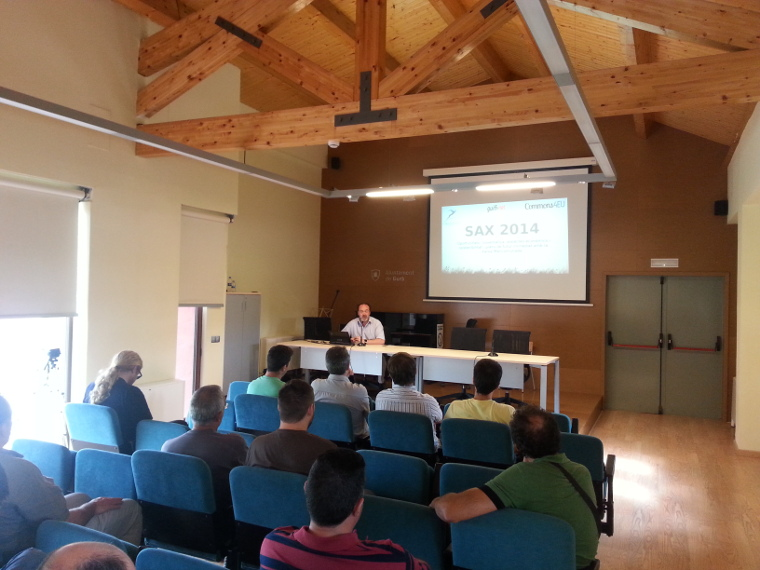
\includegraphics{sect2/figures/user_con1.jpg}} &
      \resizebox{0.465\linewidth}{!}{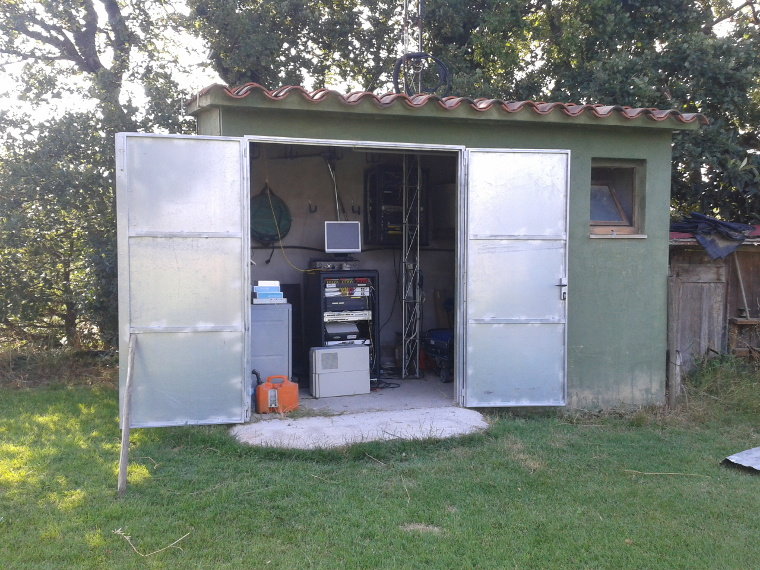
\includegraphics{sect2/figures/user_con2.jpg}} \\
      \resizebox{0.465\linewidth}{!}{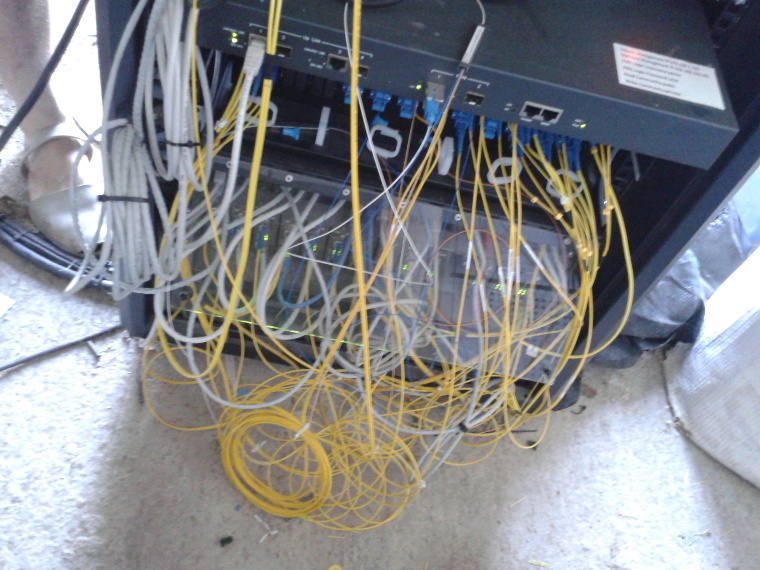
\includegraphics{sect2/figures/user_con3.jpg}} &
      \resizebox{0.465\linewidth}{!}{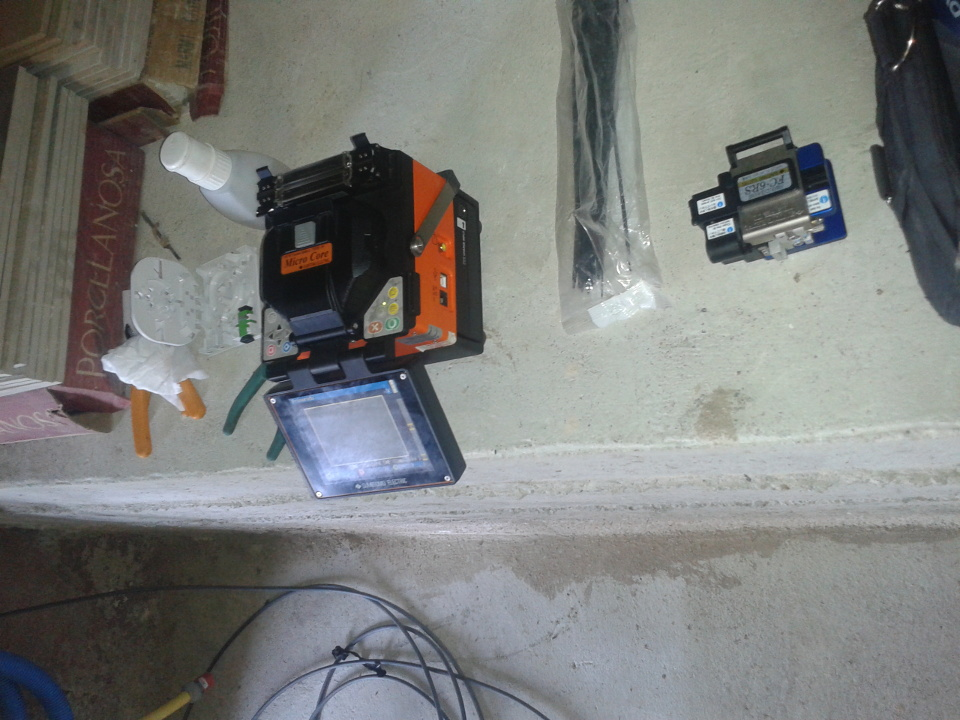
\includegraphics{sect2/figures/user_con4.jpg}} \\
    \end{tabular}
  \caption[Gurb pilot - FFTH process pictures]{Gurb pilot - Fiber From The Farm (FFTH) process pictures . Top left: Project's presentation to the neighbours. Top right: Grub's PoP general veiw. Bottom left: Backside of one of the racks of the PoP. Bottom right: The fibre splicer and the additional tools needed.}
  \label{fig:gurb_user_con}
\end{figure}

\figurename~\ref{fig:gurb_2014_transit} shows the traffic the Gurb's PoP. A clear increase can be observed since the first week of August, when the deployments done during the spring and the beginning of summer where finally put in service\footnote{The jump of the inbond traffic is mostly due to a reconfiguration of the ports monitored which was made in conjunction with the illumination of the new tracks, thus, most of does not correspond a real traffic increase.}.

\begin{figure}[H]
  \centering
  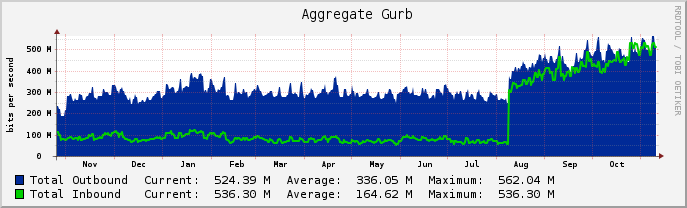
\includegraphics[width=0.95\linewidth]{sect2/figures/gurb_2014_transit.png}
  \caption[Gurb pilot: Network traffic 2014]{Gurb's pilot network traffic 2014.}
  \label{fig:gurb_2014_transit}
\end{figure}


\FloatBarrier
\subsubsection{Vic}
\label{dep_vic}

This urban deployment was started as the result of the collaboration of individuals, industries and social services. During 2013 a primary and a secondary school, a hospital and a chemical factory together with a dozen of dwelling houses have been connected. The number of connections in 2014 was expected to significantly increase. Nonetheless, due to the conflicts caused by a professional which quitted guifi.net the expansion slowed down. Solving these conflicts consumed great efforts because he involved the municipality and other actors such as the collocation centre managers. The positive outcome is that the access to the municipal fibres\footnote{Vic council constituted as operator and is deploying dark fibre. The monthly cost of a circuit within a radius of 1km is 25€/month. Ducts can also be rented at a yearly cost 1.35€/m with 80\% of reduction if they are used to deploy infrastructure held in commons.} have been standardised and thanks to it the expansion has been restarted. As \figurename~\ref{fig:map_gurbVic_2014} shows that three circuits of the municipality are already used and another three are foreseen to be used in the coming months.

\figurename~\ref{fig:map_vic_2014} shows the current deployments in green, the circuits of the municipality used or to be used in purple and the deployments planned for the coming months in yellow.

\begin{figure}[H]
  \centering
  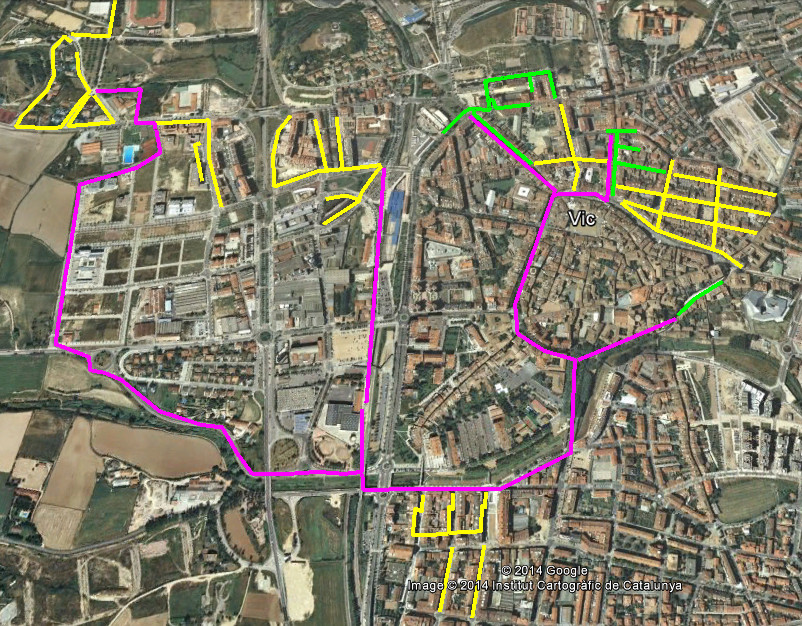
\includegraphics[width=0.95\linewidth]{sect2/figures/map_vic_2014.jpg}
  \caption[Vic pilot - OF deployment]{Green are lines are existing fibres by October 2014. Yellow ones are planned deployments to be executed before May 2015. Purple lines are circuits owned by the municipality of Vic.}
  \label{fig:map_vic_2014}
\end{figure}


%\begin{figure}[H]
%  \centering
%    \begin{tabular}{cc}
%      \resizebox{0.465\linewidth}{!}{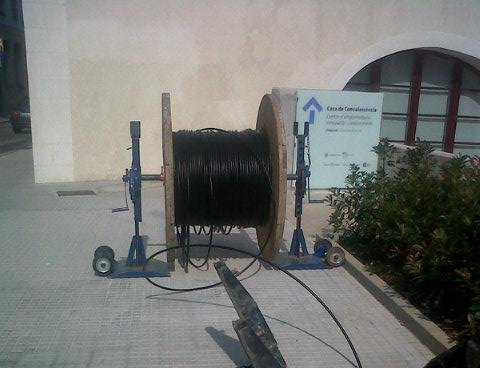
\includegraphics{sect2/figures/20130702_vic_fibra_optica_guifi_net.jpeg}} &
%      \resizebox{0.465\linewidth}{!}{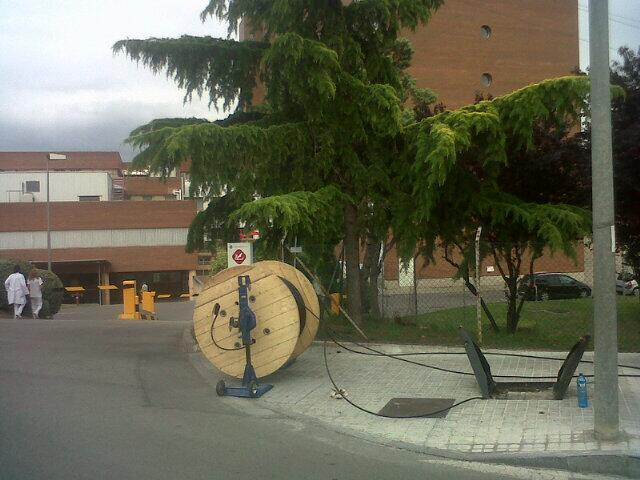
\includegraphics{sect2/figures/20130703_vic_fibra_optica_guifi_net.jpeg}} \\
%      \resizebox{0.465\linewidth}{!}{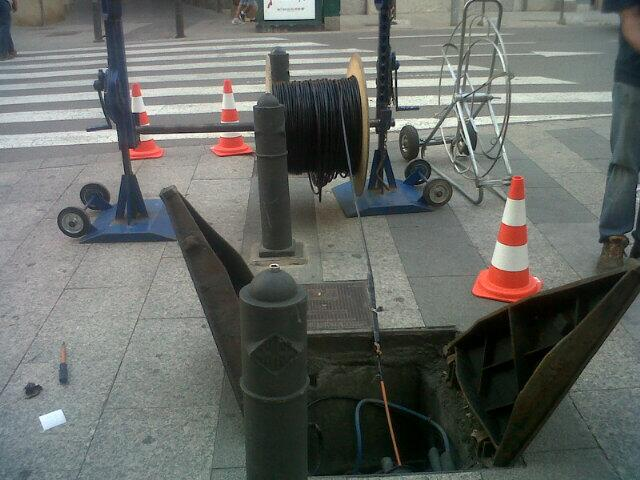
\includegraphics{sect2/figures/20130718_vic_fibra_optica_guifi_net.jpeg}} &
%      \resizebox{0.465\linewidth}{!}{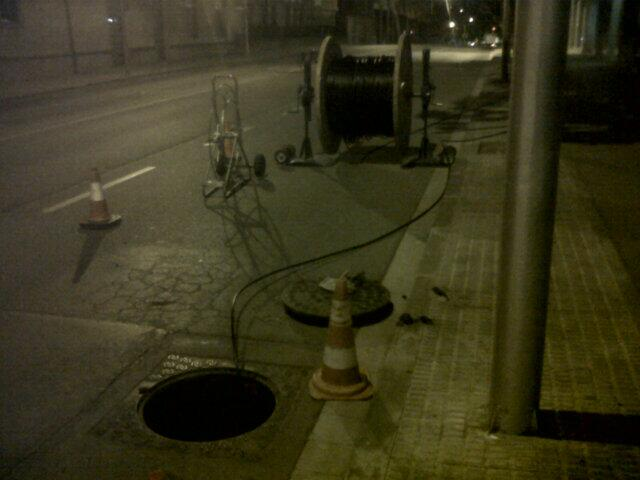
\includegraphics{sect2/figures/20130704_vic_fibra_optica_guifi_net.jpeg}} \\
%    \end{tabular}
%  \caption[Vic pilot: Connecting a hospital in an urban area]{Connecting a hospital in an urban area. Top left: The fibre reel close to the Hospital's main entrance. Top right: Already outside the Hospital venue. Bottom left: Along the streets. Bottom right: Working until late at night.}
%  \label{fig:vic_user_con}
%\end{figure}

\figurename~\ref{fig:vic_2014_transit} shows the traffic at Vic's PoP. The valleys correspond to the weekends, showing that these deployments are mostly professional (industries, schools, etc.).

\begin{figure}[H]
  \centering
  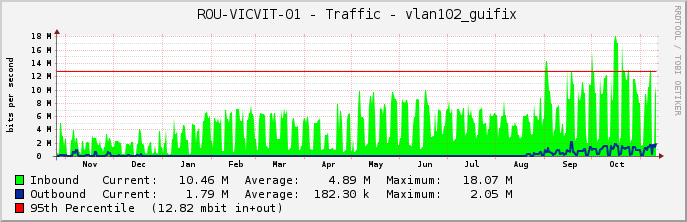
\includegraphics[width=0.95\linewidth]{sect2/figures/vic_2014_transit.png}
  \caption[Vic pilot: Network traffic 2013]{Vic's pilot network traffic 2013.}
  \label{fig:vic_2014_transit}
\end{figure}


\FloatBarrier
\subsubsection{Rub\'{i}}
\label{dep_rubi}

As already detailed in the first report, by the end of the first year this pilot was considered to be in a blocked state. In 2013 on the one hand the traditional ISPs have continued deploying their own OF, but on the other hand new opportunities to deploy BuB OF appeared. Indeed, in June a person from the city advised by the local government contacted the guifi.net Foundation to get further information about the BuB model and to discuss on the viability of setting up a consumers cooperative ISP inspired by the experience she gained during her contribution to Som Energia\footnote{\url{http://www.somenergia.coop/welcome-to-som-energia}}, an energy consumers cooperative that promotes the fair and green energies consumption.

Som Energia/Eticom\footnote{\url{http://www.eticom.coop/en/} and \url{http://www.somconnexio.org/}}, the consumers cooperative ISP, was created in March 2014 and is still in a transient state. Nevertheless, it already has over 450 hundred members and has several delegations around Spain. Despite they have not made any deployment yet, the model is very promising as well as the results already achieved. According to this model, the member fees are to be used to undertake OF deployment projects of infrastructure to be held in commons. At the same time, the coop acts as a reseller of other telecommunications companies to be able to offer a full telecommunications service set (i.e. mobile and fix data and voice) to its members. The providers are selected according to the coop ethical principles.

\FloatBarrier
\subsection{Other deployments}
\label{dep_other}

The FO initiatives in side guifi.net that consolidated during this last reporting period are:
\begin{itemize}
  \item Sant Bartomeu del Grau
  \item Cardedeu
  \item Vilafranca
  \item Sant Vicen\c{c} dels horts
  \item Sallent
\end{itemize}

Thus, guifi.net accounts for a total of 12 consolidated OF initiatives\footnote{The already consolidated before starting this reporting period are: Masquefa, Igualda, Manresa, l'Aldea, Tortosa.}
